\section{写法初探}
\begin{frame}[fragile]
    \frametitle{基本语法}
    \begin{itemize}
        \item 命令以 \verb|\| 开头,区分大小写
              \begin{lstlisting}
            \Order[option]{arg}
        \end{lstlisting}
        \item 注释以 \verb|%| 开头
        \item 环境
              \begin{lstlisting}
            \begin{env}
                ...
            \end{env}
        \end{lstlisting}
        \item 空行=段落,多个空格=一个空格
        \item 宏语言,自定义写法
    \end{itemize}
\end{frame}

\begin{frame}[fragile]
    \frametitle{文件结构}
    \scriptsize
    \begin{lstlisting}
\documentclass{ctexart}% 指明文档类型:支持中文的文章
\usepackage{amsmath,amssymb,physics}% 引入必要的宏包
\newcommand{\Key}[1]{\textbf{#1}}% 可以自定义命令
\begin{document}% 正文从下面开始
\section{格子Boltzmann方法} % 第一节标题
要想对Boltzmann-BGK方程使用计算机程序求解,势必要对其进行离散化,格子Boltzmann方程即离散化的Boltzmann-BGK方程,即
\begin{equation} % 带编号的公式
    \pdv{f_\alpha}{t}+\va*{e}_\alpha\cdot\nabla f_\alpha=-\frac{1}{\tau_0}\left(f_\alpha-f_\alpha^{\rm eq}\right)+\left(\va*{a}\cdot\nabla_{\xi}f\right)_\alpha
\end{equation}
这种离散处理将流体视为大量离散的粒子,每个粒子都会安排在一个\Key{规定好的格子Lattice}上,并按照格子的规则进行迁移,即碰撞和运动。此时,不仅空间是离散的,时间和速度也是离散的。
\end{document} % 正文在这里结束
    \end{lstlisting}
\end{frame}

\begin{frame}{文件结构}
    \begin{figure}
        \centering
        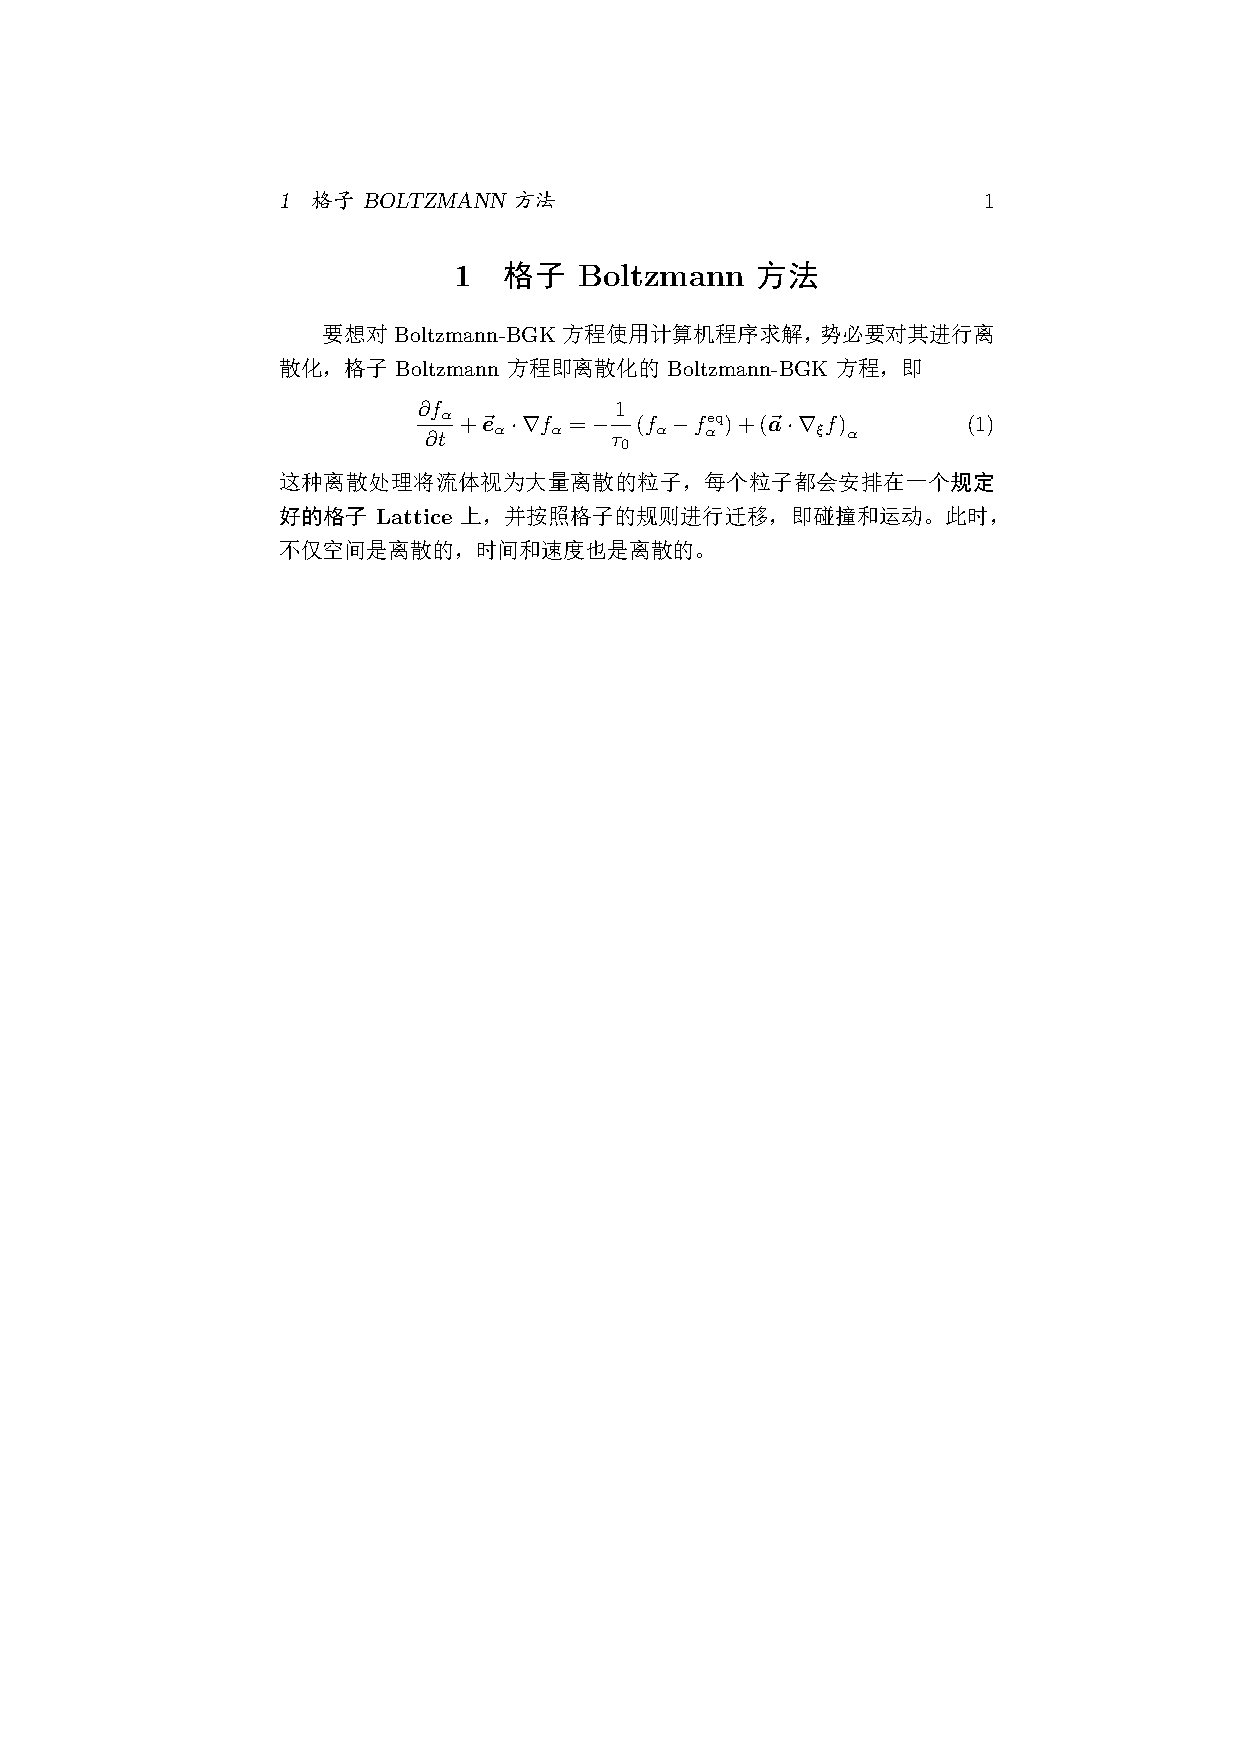
\includegraphics[scale=0.7]{figures/test2.pdf}
    \end{figure}
\end{frame}

\begin{frame}[fragile]
    \frametitle{谋篇布局}
    \begin{itemize}
        \item 文档结构
              \begin{itemize}
                  \item 标题:\verb|\title|、\verb|\author|、\verb|\date| $\to$ \verb|\maketitle|
                  \item 摘要:\verb|abstract| 环境
                  \item 目录:\verb|\tableofcontents|
                  \item 章节:\verb|\chapter|、\verb|\section|、\verb|\subsection| 等
                  \item 文献:\verb|\bibliography| 或 \verb|\printbibliography|
              \end{itemize}
        \item 文档划分
              \begin{itemize}
                  \item 分文件编译:\verb|\include|、\verb|\input|
              \end{itemize}
    \end{itemize}
\end{frame}

\begin{frame}[fragile]
    \frametitle{文本标记}
    \begin{itemize}
        \item 加粗:\verb|{\bfseries ...}| 或 \verb|\textbf{...}|
        \item 倾斜:\verb|{\itshape ...}| 或 \verb|\textit{...}|
        \item 字号:\verb|\tiny|、\verb|\small|、\verb|\large|、\verb|\Large| 等
        \item 换行:\verb|\\|
        \item 缩进:\verb|\indent|
        \item 居中:\verb|\centering| 或 \verb|center| 环境
    \end{itemize}
\end{frame}

\begin{frame}[fragile]
    \frametitle{常用环境:列表}
    \begin{columns}[c]
        \begin{column}{0.5\textwidth}
            \footnotesize
            \begin{lstlisting}
\begin{enumerate}
    \item 西安交通大学的优秀学辅
    \begin{itemize}
        \item 彭康学导团
        \item 仲英学辅
        \item 钱院学辅
        \item 治学团
    \end{itemize}
    \item 吾日三省吾身
    \begin{itemize}
        \item 群内答疑乎?
        \item 共享学习链接乎?
        \item \LaTeX{}技能精进乎?
    \end{itemize}
\end{enumerate}
            \end{lstlisting}
        \end{column}
        \begin{column}{0.5\textwidth}
            \begin{enumerate}
                \item 西安交大优秀学辅
                      \begin{itemize}
                          \item 彭康学导团
                          \item 仲英学辅
                          \item 钱院学辅
                          \item 治学团
                      \end{itemize}
                \item 吾日三省吾身
                      \begin{itemize}
                          \item 群内答疑乎?
                          \item 共享学习链接乎?
                          \item \LaTeX{}技能精进乎?
                      \end{itemize}
            \end{enumerate}
        \end{column}
    \end{columns}
\end{frame}

\begin{frame}[fragile]
    \frametitle{常用环境:图片}
    \begin{columns}
        \begin{column}{0.6\textwidth}
            \begin{lstlisting}
\begin{figure}
    \centering
    % 可指定宽度、高度等选项
    
\includegraphics[scale=0.07]{figures/PKSTU-Logo.png}
    \caption{Logo of PKSTU}
    \label{fig:PKSTU-Logo}% 方便引用
\end{figure}
            \end{lstlisting}
        \end{column}
        \begin{column}{0.4\textwidth}
            \begin{figure}
                \centering
                
\includegraphics[scale=0.07]{figures/PKSTU-Logo.png}
                \caption{Logo of PKSTU}
                \label{fig:PKSTU-Logo}
            \end{figure}
        \end{column}
    \end{columns}
\end{frame}

\begin{frame}[fragile]
    \frametitle{常用环境:表格}
    \begin{columns}
        \begin{column}{0.6\textwidth}
            \scriptsize
            \begin{lstlisting}
% 导言区
\usepackage{booktabs} % 提供\toprule等命令
% 正文
\begin{table}
    \caption{彭康学导团主要群聊人数}
    \label{tab:PKSTU-members}
    % 列格式:c 居中,l 左对齐,r 右对齐
    \begin{tabular}{cc}
    \toprule
    群聊名称 & 人数 \\
    \midrule
    彭小帮2.0 & 1417 \\
    彭小帮1.0 & 1028 \\
    学导团2022成员群 & 59 \\
    \bottomrule
    \end{tabular}
\end{table}
            \end{lstlisting}
        \end{column}
        \begin{column}{0.5\textwidth}
            \begin{table}
                \small
                \caption{彭康学导团主要群聊人数}
                \label{tab:PKSTU-members}
                \begin{tabular}{cc}
                    \toprule
                    群聊名称 & 人数 \\
                    \midrule
                    彭小帮2.0 & 1417 \\
                    彭小帮1.0 & 1028 \\
                    学导团2022成员群 & 59 \\
                    \bottomrule
                \end{tabular}
            \end{table}
        \end{column}
    \end{columns}
\end{frame}